\documentclass[tikz,border=2pt]{standalone}
\usepackage{amsmath}
\usepackage{amssymb}
\usepackage{pgfplots}
\pgfplotsset{compat=1.18}
\usetikzlibrary{arrows.meta}
\begin{document}
% Sakasegawa for c = 1, E[S] = 5, C_s^2 = 4/25: E[W] = (C_a^2 + C_s^2)/2 * rho/(1-rho) * 5 for
% C_a^2 = 1/12 (uniform inter-arrival times) and C_a^2 = 1 (Poisson); at rho = 5/6 these are 73/24 and 29/2.
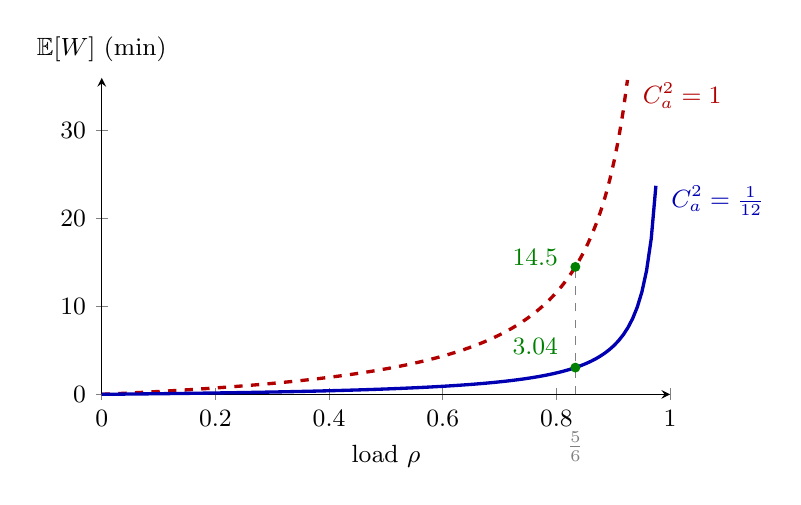
\begin{tikzpicture}[font=\small, >={Latex[length=2mm]}]
  \begin{axis}[
    axis lines=left, xmin=0, xmax=1, ymin=0, ymax=36,
    xtick={0,0.2,0.4,0.6,0.8,1}, ytick={0,10,20,30},
    xlabel={load $\rho$}, ylabel={$\mathbb{E}[W]$ (min)},
    ylabel style={rotate=-90, anchor=south, at={(axis description cs:0,1.02)}},
    samples=120, width=8.8cm, height=5.6cm, clip=false]
    \addplot[red!70!black, very thick, dashed, domain=0:0.925] {(1+0.16)/2*x/(1-x)*5};
    \addplot[blue!70!black, very thick, domain=0:0.975] {(1/12+0.16)/2*x/(1-x)*5};
    \draw[gray, thin, dashed] (axis cs:0.8333,0) -- (axis cs:0.8333,14.5);
    \fill[green!50!black] (axis cs:0.8333,14.5) circle (1.8pt);
    \fill[green!50!black] (axis cs:0.8333,3.0417) circle (1.8pt);
    \node[green!50!black, anchor=east] at (axis cs:0.82,15.6) {$14.5$};
    \node[green!50!black, anchor=south east] at (axis cs:0.82,3.4) {$3.04$};
    \node[red!70!black, anchor=west] at (axis cs:0.935,34) {$C_a^2=1$};
    \node[blue!70!black, anchor=west] at (axis cs:0.985,22) {$C_a^2=\tfrac{1}{12}$};
    \node[gray, anchor=north] at (axis cs:0.8333,-3.2) {$\tfrac{5}{6}$};
  \end{axis}
\end{tikzpicture}
\end{document}
